\chapter{Обзор современного состояния исследований накопления изотопов водорода в материалах ОПЭ}\label{ch:ch1}

\nomenclature[A, 0]{УТС}{Управляемый термоядерный синтез}
\nomenclature[A, 1]{ТЯУ}{Термоядерная установка}
\nomenclature[A, 2]{ИТЭР}{Международный экспериментынй термоядерный реактор}
\nomenclature[A, 3]{ОПЭ}{Обращенные к плазме элементы}
\nomenclature[A, 4]{DT-плазма}{Дейтерий-тритиевая плазма}
\nomenclature[A, 5]{H-мода}{Режим с высоким временем удержанием энергии в плазме токамака (High confinement regime)}
\nomenclature[A, 6]{ЛИД}{Лазерно-инудуцированная десорбция}

Исследования в области управляемого термоядерного синтеза (УТС) с магнитным удержанием плазмы достигли важного этапа, на котором длительное ($\sim100-\SI{1000}{\second}$) удержание энергии в горячей плазме становится все более реализуемо. Инженерно-техническая реализация термоядерных установок (ТЯУ) промышленного масштаба потребует решения совокупности взаимосвязанных задач для осуществления квазистационарного режима горения плазмы с параметрами, необходимыми для протекания реакции термоядерного синтеза. Ключевым аспектом продолжительной работы установок такого типа являются процессы взаимодействия пристеночной плазмы с поверхностью обращенных к плазме элементов (ОПЭ). Эти процессы существенно влияют на параметры плазмы и во многом определяют срок службы компонентов, предназначенных для защиты внутрикамерных элементов установки, что также накладывает ограничения на выбор материалов ОПЭ. Сопутствующим процессом данного взаимодействия является накопление изотопов водорода в ОПЭ. Исследование механизмов и закономерностей изотопов водорода представляет собой ключевую задачу будущих ТЯУ, использующих в качестве компонентов топлива радиоактивный тритий.

\section{Плазменные нагрузки на ОПЭ в ТЯУ}\label{sec:ch1/sec1}

% Тепловые нагрузки
Элементы первой стенки в ТЯУ на базе токамака будут подвержены воздействию интенсивных потоков тепла и частиц. В действующих установках среднее значение плотности потока тепла (отношение полной мощности, попадающей на стенку, к ее проективной площади) на ОПЭ оценивается на уровне \SIrange{0.2}{0.6}{\mega\watt\per\metre\squared}~\cite{Mazul2021}. Особенности удержания плазмы в магнитной конфигурации токамака однако приводят появлению пространственно-временного распределения этой нагрузки. Диверторная область токамаков является наиболее нагруженной. Прогностическое моделирование для строящегося токамака ИТЭР показывает, что стационарные нагрузки в нормальных разрядах\footnote{Под <<нормальными разрядами>> подразумеваются квазистационарные режимы горения плазмы, не подверженных влиянию глобальных неустойчивостей} могут достигать величины \SIrange{5}{15}{\mega\watt\per\meter\squared}~\cite{Pitts2019,Orrico2023} вблизи пересечения сеператрисы и внешних панелей дивертора, приводя к существенному нагреву поверхности до \SIrange{500}{1000}{\kelvin}.

Величина потоков тепла на ОПЭ может меняться в ходе различных переходных процессов, которые можно разделить на медленные и быстрые. К медленным можно отнести неизбежные процессы зажигания и затухания разряда длительностью около \SI{100}{\second} для ИТЭР, а также допустимые кратковременные повышения нагрузок до уровня \SI{20}{\mega\watt\per\meter\squared} длительностью в несколько секунд~\cite{Pitts2017}. Инициирование быстрых переходных процессов связано с развитием неустойчивостей разного рода~\cite{hender2007mhd}. На рисунке~\cref{fig:ch1/Heat_loads_diagram} приведена сравнительная диаграмма тепловых потоков, приходящих на диверторные пластины ИТЭР~\cite{Linke2019}.

\begin{figure}[ht]
    \centerfloat{
        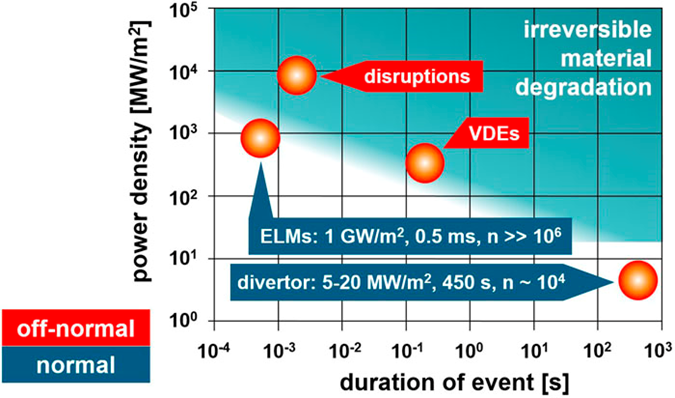
\includegraphics[scale=1]{Heat_loads_diagram.png}
    }
    \caption{Ожидаемые тепловые потоки, приходящие на ОПЭ в ИТЭР~\cite{Linke2019}. Бирюзова область соответствует области нанесения необратимого ущерба поверхности}\label{fig:ch1/Heat_loads_diagram}
\end{figure}

Значительную опасность представляют три типа событий: большие срывы тока, вертикальные смещения плазменного шнура и импульсно-периодические плазменные нагрузки во время ELM-событий. Большие срывы тока происходят при развитии глобальных магнитогидрониманических неустойчивостей. Они представляют наибольшую опасность, т.к. приводят к выбросу значительной части запасенной в плазме энергии на ОПЭ за времена порядка \SIrange{10}{100}{\milli\second}. Вертикальные смещения характерны для D-образного сечения плазменного шнура при утере устойчивости в вертикальном направлении за счет быстрых изменений параметров плазмы. События неконтролируемого вертикального смещения ведут к выходу за сепаратрису, создавая дополнительную тепловую нагрузку на ОПЭ за время порядка \SIrange{0.1}{1}{\second}. Возникновение импульсно-периодических плазменных нагрузок на ОПЭ характерно для плазменных разрядов в H-моде, переход в которую сопровождается формированием транспортного барьера на периферии плазмы. Образование транспортного барьера ведет к росту давления плазмы и его градиента на периферии пока не будет достигнут предел магнитогидрониманической устойчивости~\cite{Leonard2014}. Возникающая в результате неустойчивости (ELM-неустойчивости) вызывает быструю релаксацию давления с выбросом потока плазмы, содержащего порядка процента запасенной энергии в плазме, на ОПЭ за время \( \sim\SIrange{0.1}{1.0}{\milli\second} \). Согласно оценкам~\cite{Loarte2003, hender2007mhd, Pitts2017, Pitts2019}, потоки тепла во время переходных процессов в ИТЭР могут достигать $\sim\SI{10}{\giga\watt\per\meter\squared}$. Воздействие мощных плазменных потоков во время описанных переходных процессов может нанести серьезный ущерб поверхности (растрескивание, плавление, испарение и т.д.). Предотвращение возможного ущерба является приоритетной задачей, для решения которой разрабатываются соответствующие операционные системы и подходы~\cite{Lang2013,Evans2013,Lehnen2015}. Ввиду этого, далее в работе основное внимание будет уделено переходным процессам типа ELM-событий, последствия развития которых предполагаются либо допустимыми, либо могут быть минимизированы до приемлемого уровня.

Потоки частиц, приходящие на ОПЭ в действующих установках, в основном состоят из электронов, ионов и нейтралов перезарядки изотопов водорода. Возможно также наличие малой доли примеси более тяжелых атомов/ионов материалов ОПЭ, остаточного газа или примесей, вводимых в установку для кондиционирования стенок или распределения тепловых нагрузок. В проектируемых ТЯУ, в т.ч. и токамаке ИТЭР, корпускулярные нагрузки также будут включать продукты DT-реакции синтеза: высокоэнергетичные нейтроны (\SI{14.1}{\mega\electronvolt}) и альфа-частицы (\SI{3.5}{\mega\electronvolt}). Длительные режимы работы установок будут сопровождаться высокой дозой облучения ОПЭ, что также может приводить к модификации как поверхностной, так и объемной структуры. К тому же, важней задачей с точки зрения обеспечения радиационной безопасности является минимизация накопления радиоактивного трития в элементах установки на протяжении ее срока эксплуатации.

Плотность потока частиц на элементы первой стенки ИТЭР оценивается на уровне \SIrange{e18}{e20}{\particles\per\metre\squared\per\second}~\cite{DeTemmerman2021, Rivals2022}, когда для диверторных пластин "--- на уровне \SIrange{e23}{e24}{\particles\per\metre\squared\per\second}~\cite{Pitts2019,Orrico2023}, причем энергия приходящих ионов составляют величину порядка \SIrange{1}{100}{\electronvolt}. Оценка суммарной дозы облучения пластин дивертора в ИТЭР показывает, что за 5000 номинальных разрядов длительностью \SI{400}{\second} ее величина составит \( \sim \SIrange{e29}{e30}{\particles\per\metre\squared} \). Как показано на сравнительных диаграммах на рисунке~\cref{fig:ch1/fluxes_comparison}, условия эксплуатации ОПЭ в ИТЭР будут намного суровее, чем в действующих установках по исследованию магнитного удержания плазмы.
\begin{figure}[ht]
    \centerfloat{
        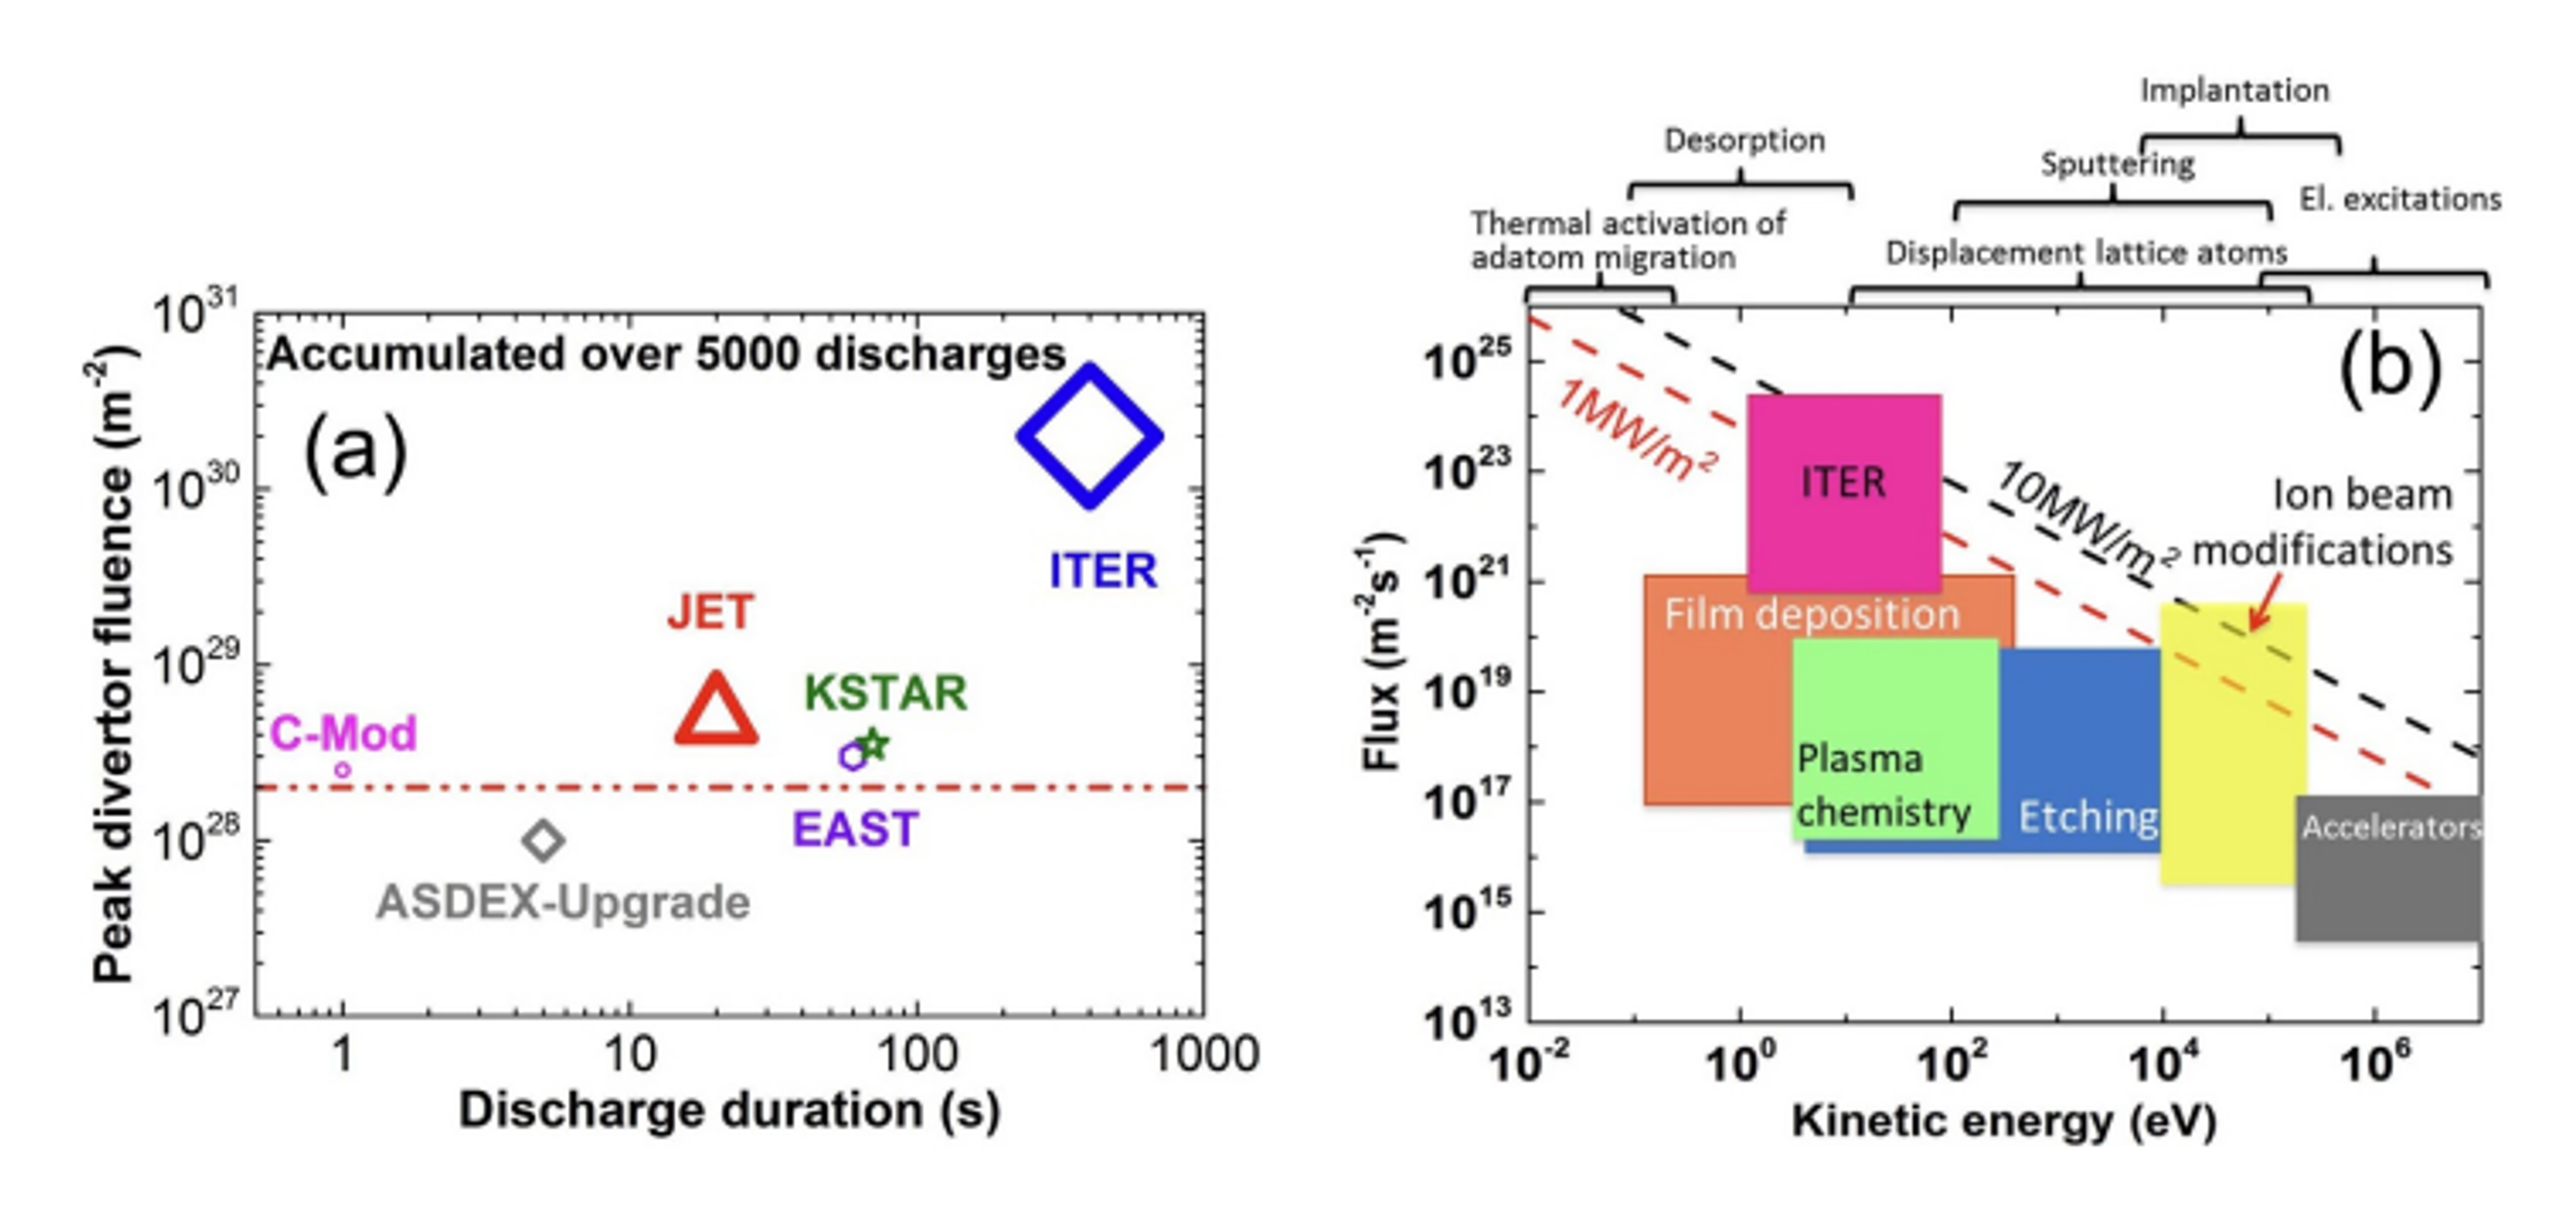
\includegraphics[scale=0.9]{fluxes_comparison.png}
    }
    \caption{Сравнение оцененной ионной дозы после 5000 тысяч нормальных плазменных разрядов в различных токамаках (слева) и характерных условий облучения в различных типах экспериментов~\cite{DeTemmerman2018}}\label{fig:ch1/fluxes_comparison}
\end{figure}
Энергии ионов в диверторе сопоставимы с энергиями, используемыми в различных методах плазменного осаждения и травления, однако плотности потока ионов и энергии на несколько порядков выше. Помимо этого, поток и энергия ионов, приходящих на поверхность ОПЭ, могут увеличиваться во время переходных процессов. Анализ данных с диагностических систем (зонды Ленгмюра и \(\mathrm{D}_\alpha\)-спектроскопия) токамака JET~\cite{Guillemaut2015,Guillemaut2018} демонстрирует кратное увеличение измерительных сигналов во время ELM-событий, что косвенно соответствуют пропорциональному росту потока частиц. Считается, что энергия частиц во время ELM-событий пропорциональна температуре плазмы на пьедестале~\cite{Eich2017}. При сохранении аналогичных зависимостей для токамака масштаба ИТЭР можно ожидать соответствующее превышение уровня стационарных нагрузок с энергия приходящих ионов порядка нескольких килоэлектронвольт.

Немаловажным остается влияние образования гелия и нейтронов на эксплуатацию ОПЭ. Генерируемы в ходе DT-реакции частицы гелия должны терять большую часть своей энергии в центре плазменного шнура, однако стационарное облучение материалов ионами гелия с низкой энергией также может оказывать существенное влияние. Известно, что облучение тугоплавких металлов ионами гелиевой плазмы индуцирует формирование гелиевых пузырей в объеме материала, а также может приводить к его структурным изменениям с образованием высокопостристых структур~\cite{Ueda2018,Kajita2018,Fedorovich2019}. Любые незапланированные структурные изменения морфологии поверхности ОПЭ будут влиять на процессы взаимодействия плазмы с ней, что может приводить к глобальным изменениям в режимах удержания плазмы.

Взаимодействие ионов с ОПЭ носит поверхностный характер. Падающий на поверхность поток частиц может приводить либо к обратной эмиссии частиц (отражение, распыление), либо к их имплантации. Средняя глубина внедрения частиц (за исключением эффектов каналирования) может достигать нескольких десятков нанометров в зависимости от состава и структуры мишени, сорта приходящих частиц и их энергии~\cite{eckstein2010penetration}. Ввиду гораздо большей глубины пробега нейтронов основные процессы взаимодействия происходят в объеме материалов. Облучение нейтронными потоками ведет к объемному нагреву материалов, их трансмутации, а также образованию дефектов кристаллической решетки за счет развития каскадов столкновений. Прогнозируемый уровень повреждений в конце срока службы токамака ИТЭР оценивается гораздо ниже инженерных ограничений~\cite{Villari2013}. Тем не менее, образование радиационных дефектов в материалах ОПЭ в ходе работы установки может влиять на удержание изотопов водорода.

\section{Материалы ОПЭ в ТЯУ}\label{sec:ch1/sec2}

Влияние описанных в предыдущим разделе отдельных типов нагрузок широко исследовалось в лабораторных условиях (исключением могут служить эффекты, связанные с облучением нейтронам с МэВ-ной энергии). В общем случае, они будут оказывать совместное влияние, что качественно проиллюстрировано на рисунке~\cref{fig:ch1/synergetic_diagram}. Синергетические эффекты воздействия на ОПЭ в не достижимых ранее условиях ТЯУ могут создавать новые вызовы для выбора их оптимальной конструкции.
\begin{figure}[ht]
    \centerfloat{
        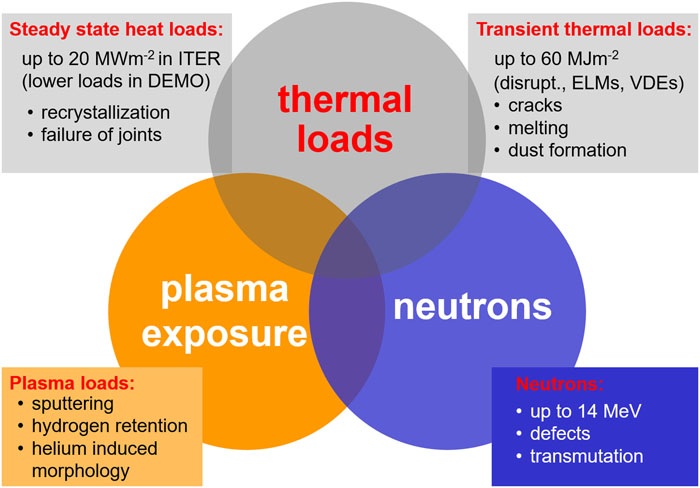
\includegraphics[scale=0.5]{synergetic_diagram.png}
    }
    \caption{Синергетические нагрузки и их основные последствия для ОПЭ при работе ТЯУ~\cite{Linke2019}}\label{fig:ch1/synergetic_diagram}
\end{figure}
Эти аспекты также накладывает совокупность требований и на выбор используемых материалов. К основным факторам, определяющим этот выбор, можно отнести термостойкость и теплопроводность, эрозионную устойчивость при ионном облучении, способность накапливать изотопов водорода, устойчивость и низкую активируемость при нейтронном облучении. Высокая термостойкость и теплопроводность, а также низкая эрозия при облучении легкими ионами характерны для тугоплавких металлов с большим зарядовым числом ядра ($Z$). Однако распыление и попадание в область горячей плазмы атомов таких материалов может приводить к увеличению потерь мощности на излучение из плазмы~\cite{Ptterich2019}. Более легкие материалы подвержены большей эрозии поверхности и могут влиять на динамику накопления изотопов водорода в ТЯУ. \nomenclature[P,00]{$Z$}{Атомный номер элемента}

Основными материалами, применяемыми в современных установках, являются графит (JT-60SA~\cite{Shirai2024}, T-15МД~\cite{Velikhov2024}), бериллий (JET~\cite{Maggi2024,Kappatou2025}), молибден(EAST~\cite{Gong2024}) и вольфрам (JET, EAST, WEST~\cite{Shi2025}, ASDEX-Upgrade~\cite{Rohde2009}). Углеродные материалы являются привлекательным выбором для ОПЭ ввиду ряда преимуществ. Проникновение углерода в плазму ведет к малым потерям мощности с излучением из-за его низкого зарядового числа ($Z=6$). Углеродные материалы характеризуются высокими теплостойкостью и значением теплопроводности ($\SIrange{100}{300}{\watt\per\meter\squared\per\kelvin}$ при комнатной температуре~\cite{Merola2004, Begrambekov2023}), сопоставимой с металлами. Помимо этого, нагрев поверхности до высоких температур (>\SI{3800}{\kelvin}) ведет к сублимации материала, а не плавлению, что предотвращает вероятность развития процессов взаимодействия расплава с приповерхностной плазмой и магнитным полем. Однако углеродные материалы более подвержены распылению при облучению легкими ионами, чем, например, вольфрам. а также характеризуются высоким коэффициентом химического распыления при облучении изотопами водорода. Для сравнения на рисунке~\cref{fig:ch1/sputerring_yields} приведены расчетные коэффициенты распыления углерода (физического и химического), бериллия и вольфрама. Влияние химического распыления может быть минимизировано обеспечением <<благоприятного>> режима облучения, но другим важным недостатком углеродных материалов является накопление изотопов водорода. Изотопы водорода образуют прочные C-H связи, что может приводить к чрезмерному накоплению трития в переосажденных пленках и затруднять извлечению трития из установки~\cite{Gasparyan2024}. Помимо этого, интенсивное облучение потоками нейтронов и компонентов плазмы может приводить к деградации теплофизических свойств~\cite{Wu1994} и структурным изменениям поверхностных слоев~\cite{Wang2018,Begrambekov2019,Seyedhabashi2025}.

\begin{figure}[ht]
    \centerfloat{
        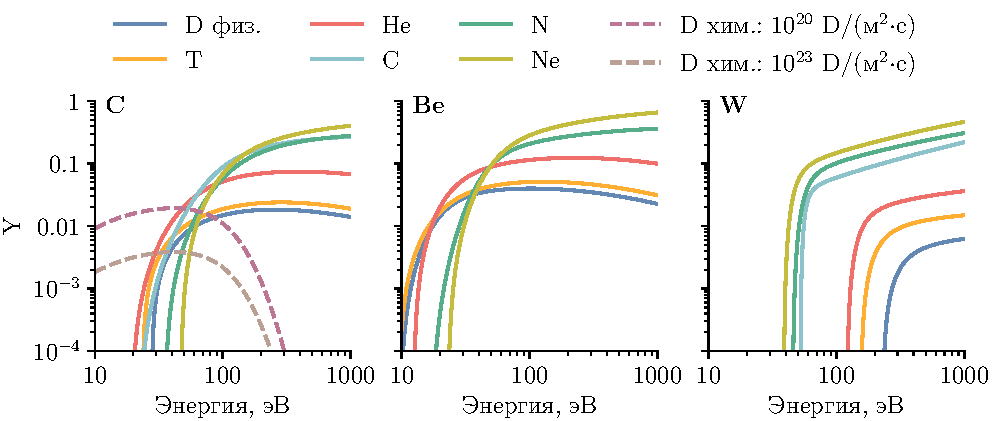
\includegraphics[scale=1]{sputerring_yields.pdf}
    }
    \caption{Расчетные зависимости коэффициентов физического распыления бериллия, углерода и вольфрама от энергии некоторых типов ионов при нормальном падении~\cite{international2001iaea, behrisch_2025}. Для углерода также приведены зависимости коэффициента химического распыления дейтерием при комнатной температуре и различных значениях потока~\cite{Roth1999,Roth2004}}\label{fig:ch1/sputerring_yields}
\end{figure}

Бериллий, как и углерод, обладает низким атомным номером ($Z=4$), что обеспечивает относительно хорошую совместимость за счет минимизации потерь мощности на излучения при проникновение бериллия в область горячей плазмы. Он также обладает высокой теплопроводностью (\SI{200}{\watt\per\meter\per\K}) и относительно высокой температурой плавления (\SI{1560}{\kelvin})~\cite{Ho1974}. По сравнению с углеродными материалами, скорость химического распыления~\cite{Brezinsek2014} и накопления изотопов водорода~\cite{DeTemmerman2021} в нем существенно меньше. Переход к металлической облицовке в токамаке JET привел к снижению интегральной эрозии ОПЭ и, как следствие, накоплению изотопов водорода~\cite{Brezinsek2015}. Бериллий также химически активен, что позволяет эффективно связывать кислород. Не смотря на явные преимущества бериллия как материала для ОПЭ, он обладает рядом существенных недостатков. Первым из них является токсичность бериллиевой пыли, что требует применения специальных мер по работе с ним~\cite{Strupp2011}. Вторым недостатком является низкая энергия связи атомов кристаллической решетки, что приводит к более высокому коэффициенту физического распыления по сравнению с графитом (рис.~\cref{fig:ch1/sputerring_yields}) и, соответственно, меньшему сроку службы под действием интенсивного ионного облучения. Следующим негативным свойством является деградация теплофизических свойств и охрупчивание бериллия, являющееся синергетическим эффектом облучения потоками нейтронов и гелия~\cite{Kesternich2003,Gilbert2012}. Последним является малая температура плавления по сравнению с иными материалами, что ограничивает использование бериллия в высоконагруженных областях установки без активного охлаждения. Совокупность этих и иных особенностей послужили причиной принятия решения об отказе от использования бериллия в качестве ОПЭ токамака ИТЭР~\cite{Barabaschi2025}, однако использование бериллия рассматривается для российского токамака ТРТ~\cite{Mazul2021,Piskarev2024}.

Молибден ($Z=42$) и вольфрам ($Z=74$) являются тугоплавкими металлами с высокими температурами плавления: \SI{2896}{\kelvin} и \SI{3695}{\kelvin}, соответственно. Однако вольфрам предпочтительнее по причине более высоких эксплуатационных характеристик, хоть и обладает рядом свойств усложняющих технологическое производство элементов облицовки с ним~\cite{Piskarev2024}. Исходя из этого, основное внимание будет уделено вольфраму. Помимо высокой теплостойкости, вольфрам характеризуется низким коэффициентом распыления легкими ионами (рис.~\cref{fig:ch1/sputerring_yields}), совместимостью с нейтронным облучением и низкой растворимостью изотопов водорода~\cite{Pintsuk2012,Rieth2019}. Явным недостатком вольфрама является вероятность распыления тяжелыми примесными ионами в плазме или ее легкими основными компонентами с высокой энергией, сопровождаемое загрязнением плазмы частицам с высоким атомным номером. Как отмечалось в разделе~\cref{sec:ch1/sec1}, потоки частиц плазмы с высокой энергией ожидаются в ходе различных переходных процессов. Известна также проблема образования трещин на поверхности вольфрама при циклических тепловых нагрузках, характерных для ELM-событий. Дополнительно необходимо отметить активно исследуемые в последнее время изменения поверхности вольфрама при облучении ионами гелиевой плазмы. В условиях, характерных для диверторной области токамаков, облучение ионами гелия ведет к формированию высокопористой наноструктуризованной морфологии, называемой <<пух>>~\cite{Ueda2018,Kajita2018,Fedorovich2019,hammond2017helium,Kajita2020,Wright2022}. Рост вольфрамового <<пуха>> на поверхности может повысить вероятность зажигания униполярных дуг с соответствующем увеличением уровня эрозии поверхности. Невзирая на недостатки вольфрама, он выбран в качестве основного материала ОПЭ для ИТЭР~\cite{Pitts2025} и находится в приоритетном списке как для ТРТ~\cite{Piskarev2024}, так и для других установок, проектируемых в настоящее время.


Учитывая риски появления тяжелой примеси в горячей плазме при распылении вольфрама, рассматривается применения различных материалов для нанесения кондиционирующих покрытий. Двумя распространенными материалами, применяемыми в действующих установках, являются литий ($Z=5$) и бор ($Z=3$). Оба материала обладают низким атомным номером и являются химически активными по отношению к кислороду и углероду, что позволяет снизить долю более тяжелой примеси в плазме~\cite{Winter1996,Wauters2020}. С другой стороны, более высокая скорость эрозии покрытий требует применения методов их регулярного обновления. Тем не менее, эксперименты на токамаках ASDEX-Upgrade~\cite{Krieger2023} и EAST~\cite{Yu2023} продемонстрировали, что применении легких материалов для кондиционирования стенок может обеспечить режимы плазменных разрядов с низким рециклингом изотопов водорода, что может привести к осуществлению длительных стабильных разрядов~\cite{Zakharov2019}. Помимо методов нанесения защитных покрытий, ведется активное развитие альтернативных вариантов, например самопассивируемые сплавы вольфрама с пониженным термоокислением~\cite{Litnovsky2020} и капиллярно-пористые системы с жидкими металлами~\cite{Lublinskii2015}, которые, возможно, решат проблемы, характерные для традиционных материалов.

\section{Накопление изотопов водорода в вольфраме}

Как показно в предыдущем разделе, вольфрам обладает совокупностью свойств, определяющим его применимость в качестве материала ОПЭ. Перспектива его использования инициировала всестороннее изучение закономерностей накопления изотопов водорода в условиях, ожидаемых в ТЯУ. Необходимость детального анализа во многом обусловлена необходимостью контроля за содержанием радиоактивного трития. Так, для токамака ИТЭР установлен административный лимит в \SI{700}{\gram} по интегральному накоплению в элементах вакуумной камеры с учетом возможных погрешностей и накопления в крионасосах~\cite{Roth1}. В данном разделе приведены основные механизмы и экспериментальные результаты исследования накопления изотопов водорода в вольфраме.

\subsection{Механизмы накопление изотопов водорода в ТЯУ}

Изотопы водорода могут накапливаться на поверхности ОПЭ за счет адсорбции низкоэнергетичных атомов или молекул. Совокупность каналов адсорбции является процессом динамического (краткосрочного) удержания и не представляет особой проблемы, т.к. дегазация поверхности протекает достаточно быстро при повышенных температурах. Выделяют два основных канала долгосрочного удержания изотопов водорода: захват в объеме материала и соосаждение~\cite{Gasparyan2024, Skinner2009}. Также можно отметить накопление изотопов на поверхности или в объеме пылевых микрочастиц, образующихся в процессе эрозии поверхностных слоев ОПЭ. Накопление в пылевых частицах сильно зависит от механизма их образования и во многом может описываться процессами, определяющими захват водорода в объеме ОПЭ или при соосаждении. В силу этого, основное внимание будет уделено двум другим процессам долгосрочного удержания изотопов водорода в ТЯУ.

Основные процессы, определяющие долгосрочное накопление, схематически представлены на рисунке~\cref{fig:ch1/retention_mechanisms}.
\begin{figure}[ht]
    \centerfloat{
        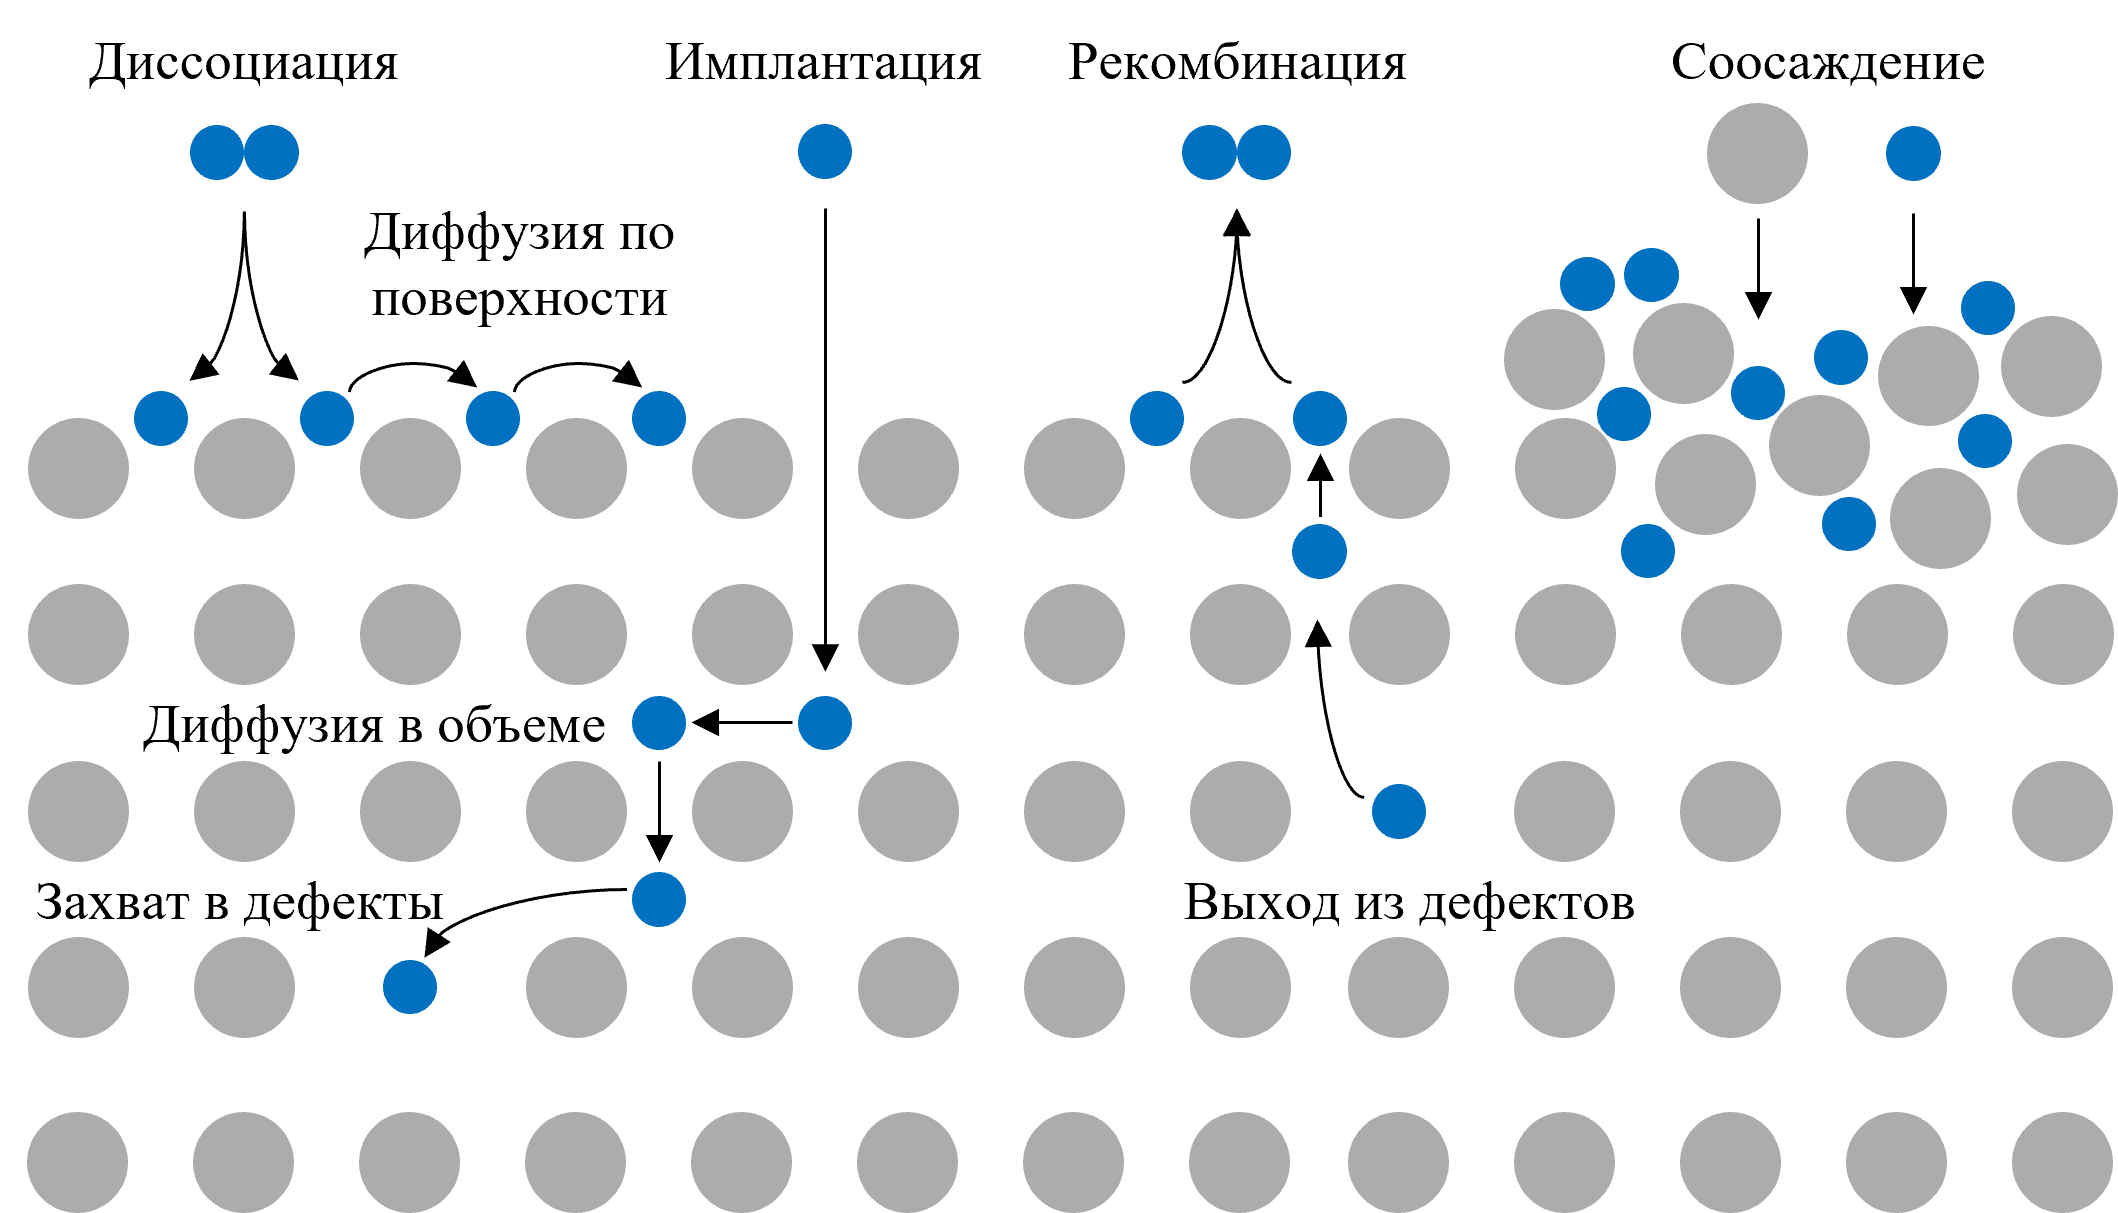
\includegraphics[scale=1]{retention_mechanisms.png}
    }
    \caption{Схематическое представление процессов захвата изотопов водорода при имплантации и соосаждении. Синие круги соответствуют атомам водорода, серые "--- атомам облучаемого материала}\label{fig:ch1/retention_mechanisms}
\end{figure}
Захват изотопов водорода при ионном облучении изначально происходит за счет имплантации частиц. Вероятность внедрения ионов определяется интегральным коэффициентом отражения, зависящим от параметров облучения и сортов взаимодействующих частиц. При попадании в объем внедренные частицы продолжают движение, теряя свою начальную энергию за счет упругих и неупругих потерь, пока не термализуются. Подвижность атомов водорода в металлах, как вольфрам, остается достаточно высокой при повышенных температурах, что позволяет им диффундировать обратно к поверхности и десорбироваться за счет различных процессов, например рекомбинации. С другой стороны, характерная глубина внедрения ионов в условиях токамака не превышает десятков нанометров. Интенсивное облучение поверхности приводит к быстрому насыщению водорода в зоне имплантации, что инициирует распространение водорода вглубь материала. В ходе диффузии подвижные атомы водорода могут захватываться различными дефектами кристаллической решетки, представляющие собой более глубокие потенциальные ямы по сравнению с межузельными положениями. Учитывая диффузионный характер накопления, величина интегрального накопления пропорциональна квадратному корню из времени (дозы) облучения, что наблюдается в многочисленных экспериментах~\cite{Ogorodnikova2003,Ogorodnikova2009,Sugiyama2014,Zhang2020}. Ввиду малой растворимости водорода в вольфраме, долгосрочное накопление будет определяться распределением и концентрацией дефектов, образование которых будет происходить при ионном и нейтронном облучении.

Процесс соосаждения водорода и материалов первой стенки в токамаках происходит в несколько итерационных этапов. Непрерывное распыление материалов ОПЭ приводит к попаданию примесных атомов в плазму, в которой они ионизуются. Ионы материалов стенки за счет процессов переноса в пристеночной плазме в итоге нейтрализуются и осаждаются на других элементах облицовки, инициируя рост поверхностных пленок. В то же время осаждаемые пленки подвергаются непрерывному облучению потоками частиц из плазмы. Совместное протекание обоих процессов ведет к практическому равномерному накоплению изотопов водорода, интегральная величина которого растет приблизительно линейно с временем. Важно заметить, что накопление изотопов водорода в процессе совместного соосаждения также сопровождается всеми процессами, характерными при имплантации в объем.

Результаты, полученные на современных токамаках, указывают на то, что соосаждение является доминирующим каналом накопления изотопов водорода. Параметры удержания водорода, физические свойства и скорость роста пленок сильно зависят от параметров совместного осаждения~\cite{Gasparyan2019,Krat2020,Krat2025}. Доля водорода в пленках может достигать десятков процентов для различных материалов (см. Рисунок~\cref{fig:ch1/codeposition_review}).
\begin{figure}[ht]
    \centerfloat{
        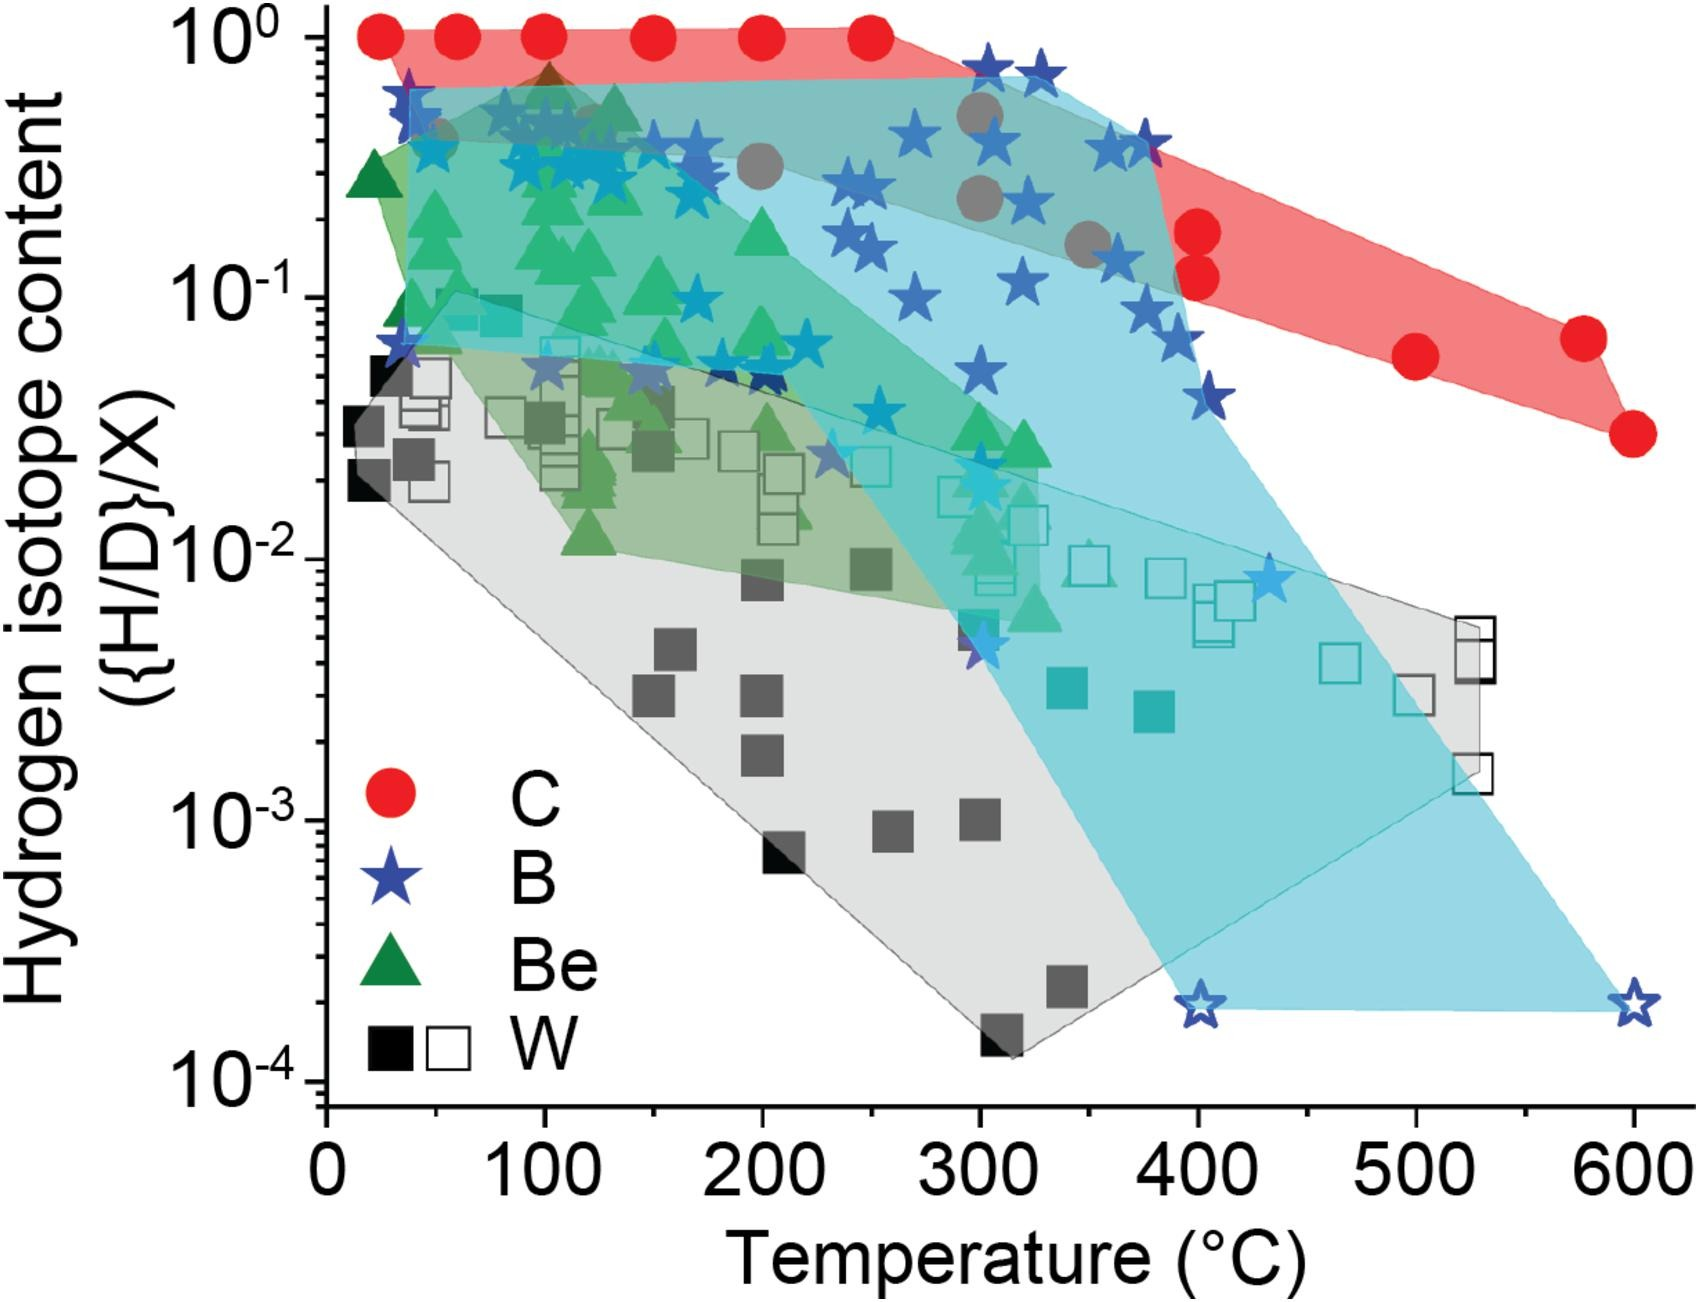
\includegraphics[scale=0.15]{codeposition_review.png}
    }
    \caption{Содержание изотопов водорода в зависимости от температуры совместного осаждения для пленок бора (голубая область), вольфрама (серая область), бериллия (зеленая область) и углерода (красная область)~\cite{Pitts2025}}\label{fig:ch1/codeposition_review}
\end{figure}
Примечательно, что содержание водорода оказывается систематически меньше в пленках вольфрама по сравнению с другими материалами. Помимо этого, скорость образования вольфрамовых пленок может быть меньше в ТЯУ из-за более высокого порога распыления. Однако недавний \textit{post-mortem} анализ образцов-свидетелей из токамака WEST указывает на образование переосажденных слоев с толщиной несколько микрометров~\cite{Bucalossi2024}.

\subsection{Взаимодействие изотопов водорода с вольфрамом}

Транспорт внедренных атомов водорода в вольфраме включает множество механизмов, которые можно разделить на несколько групп: диффузионные механизмы, взаимодействие с различными типами дефектов и поверхностные процессы. Качественное описание каждой из групп можно дать на основе одномерного представления пространственного распределения потенциальной энергии атомов водорода вблизи поверхности материала (см. рисунок~\cref{fig:ch1/potential_diagram_all}). Важно заметить, что в реальности ситуация оказывается гораздо сложнее, а распределение энергии водорода в материале с дефектами кристаллической решетки представляет из себя трехмерное пространство с совокупностью локальных экстремумов и седловых точек. Получение детальной информации о распределении потенциальной энергии возможно при помощи \textit{ab initio} методов, как теория функционала электронной плотности (DFT).

\nomenclature[A, 7]{DFT}{Теория функционала электронной плотности (Density functional theory)}

\begin{figure}[ht]
    \centerfloat{
        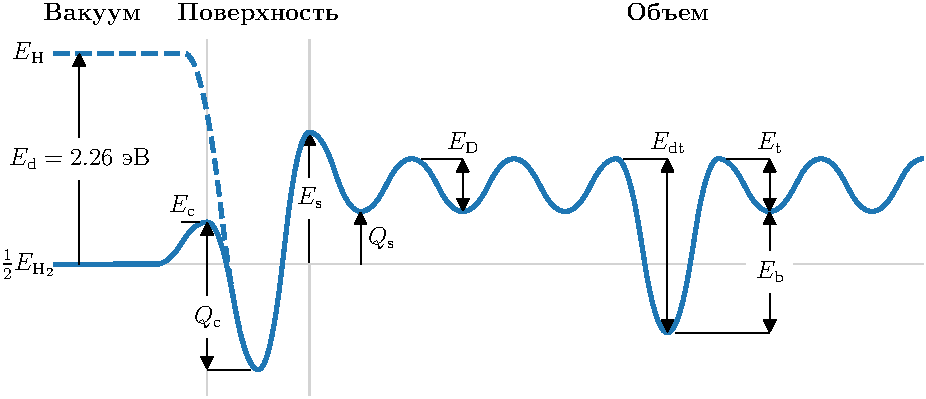
\includegraphics[scale=1]{potential_diagram_all.pdf}
    }
    \caption{Схематическая диаграмма потенциальной энергии водорода вблизи поверхности металла с положительной теплотой растворения. Уровни энергии отсчитываются от связанного состояния атома в молекуле водорода, расположенной далеко в вакууме}\label{fig:ch1/potential_diagram_all}
\end{figure}

\subsubsection{Диффузия}

Отталкивающий характер взаимодействия между атомами кристаллической решетки и водорода определяет предпочтительная оккупация последним межузульных положений, являющимися локальными минимумами потенциальной энергии. Для вольфрама с объемно-центрированной кубической решеткой наиболее устойчивыми положениями являются тетраэдрическое и октаэдрическое, причем первое является более энергетически выгодным со значение теплоты растворения $Q_\mathrm{c}$\nomenclature[P, 01]{$Q_\mathrm{s}$}{Теплота растворения [\si{\electronvolt}]} равным \SIrange{0.9}{1.0}{\electronvolt}~\cite{Heinola2010,Fernandez2015,Zhou2024}. В процессе колебаний атомы водорода могут перескакивать между равновесными положениями, распространясь стохастически по объему материала. Направления диффузионный поток атомов водорода $\mathbf{J}$ может быть обусловлен градиентами химического потенциала с вкладом $\mathbf{J}_c$ и температуры с вкладом $\mathbf{J}_T$~\cite{Longhurst1985, Krom1999, Martinez2021}:
\begin{equation}
    \mathbf{J}=\mathbf{J}_c+\mathbf{J}_T.
\end{equation}
В приближении малой концентрации растворенного водорода и отсутствия градиента напряжений в решетке вольфрама вклад от градиента химического потенциала можно редуцировать к влиянию градиента концентрации (закон Фика), определяющего поток $\mathbf{J}_{c}$:
\begin{equation}
    \mathbf{J}_{c} = -D \nabla \cm,
\end{equation}
где $D$ [\si{\meter\squared\per\second}] "--- коэффициент диффузии, $\cm$ [\si{\atoms\per\meter\cubed}] "--- концентрация атомов подвижного водорода. Диффузия, вызванная градиентом концентрации, является термоактивируемым процессом и в обычных условиях протекает быстрее с ростом температуры. Температурная зависимость коэффициента диффузии обычно описывается в соответствии с законом Аррениуса:
\begin{equation}
    D=D_0 \exp\left( -\frac{E_\mathrm{D}}{k_\mathrm{B}T} \right),
\end{equation}
где $E_\mathrm{D}$ [\si{\electronvolt}] "--- энергия активации диффузии, $k_\mathrm{B}=\SI{8.617e-5}{eV\per\kelvin}$ "--- постоянная Больцмана, $T$ [\si{\kelvin}] "--- абсолютная температура.

\nomenclature[P, 02]{$J$}{Поток атомов [\si{\atoms\per\meter\squared\per\second}]}
\nomenclature[P, 03]{$J_{c}$}{Поток атомов, индуцированный градиентом концентрации [\si{\atoms\per\meter\squared\per\second}]}
\nomenclature[P, 04]{$J_{T}$}{Поток атомов, индуцированный градиентом температуры (\si{\atoms\per\meter\squared\per\second})}
\nomenclature[P, 05]{$D$}{Коэффициент диффузии [\si{\meter\squared\per\second}]}
\nomenclature[P, 06]{$\cm$}{Концентрация подвижного водорода [\si{\atoms\per\meter\cubed}]}
\nomenclature[P, 07]{$E_\mathrm{D}$}{Энергия активация диффузии" [\si{\electronvolt}]}
\nomenclature[P, 08]{$k_\mathrm{B}$}{Постоянная Больцмана [\si{\electronvolt\per\kelvin}]}
\nomenclature[P, 09]{$T$}{Абсолютная температура [\si{\kelvin}]}

Определение коэффициента диффузии проводилось как посредством экспериментов, так и путем моделирования. Параметры коэффициента диффузии, определенные \textit{Р. Фраунфельдером} ($D_0=\SI{4.1e-7}{\metre\squared\per\second}$, $E_\mathrm{D}=\SI{0.39}{\electronvolt}$, $T=\SIrange{1100}{2400}{K}$)~\cite{frauenfelder1969solution}, продолжительное время считались наиболее надежными. Последующие результаты моделирования методом DFT~\cite{Heinola2010,Fernandez2015,Zhou2024} и недавние эксперименты~\cite{Holzner2020} указывают на большую подвижность атомов водорода в вольфраме с энергией активации диффузии в диапазоне \SIrange{0.2}{0.28}{\electronvolt}. Указанный диапазон согласуется с результатами Фраунфельдера при учете экспериментальных данных в высокотемпературной области, когда влиянием центров захвата на диффузию можно пренебречь~\cite{Heinola2010}. Тем не менее, значения коэффициента диффузии изотопов водорода сильно варьируются в литературе~\cite{remi_delaporte_mathurin_2024_13912922}, что значительно затрудняет проведение оценок накопления в материалах ОПЭ.

Облучение ОПЭ мощными тепловыми потоками неминуемо приведет к образованию температурных градиентов. Такая ситуация особо актуальна для конструкций элементов с активным водяным охлаждением, как диверторные моноблоки токамака ИТЭР. Градиент температур индуцирует поток термодиффузии $\mathbf{J}_T$ (эффект Соре):
\begin{equation}
    \mathbf{J}_{T} = -D\frac{\cm Q^*}{kT^2} \nabla T,
\end{equation}
направление которого определяется знаком теплоты переноса $Q^*$ [\si{\electronvolt}].
\nomenclature[P, 10]{$Q^*$}{Теплота переноса [\si{\electronvolt}]}

К сожалению, в настоящее время отсутствует общепринятое значение теплоты транспорта водорода в вольфраме. Экспериментальные измерения показывают, что теплота переноса в металлах с положительной теплотой растворения отрицательна и незначительно растет с температурой~\cite{Longhurst1985}. Оценки величины методом молекулярной динамики~\cite{Martinez2021,Dasgupta2023} также подтверждают отрицательное значение, но определенная функциональная зависимость обратно пропорционально квадрату температуры:
\begin{equation}
    \label{eq:ch1/heat_transport}
    Q^*=-0.0045 \kB T^2.
\end{equation}

\subsubsection{Центры захвата}

Дефекты в кристаллической решетке вольфрама, такие как вакансии, примеси, дислокации или пустоты, создают потенциальные энергетические ямы, более глубокие, чем для междоузлий. Такие дефекты являются потенциальными <<ловушками>> для подвижных атомов водорода. Захваченные в ловушки атомы становится <<иммобильным>> и могут покинуть ее, если тепловой энергии достаточно для преодоления потенциального барьера $E_\mathrm{dt}$ [\si{\electronvolt}]. Упрощенный процесс захвата можно представить в следующем виде~\cite{Drexler2020}:

\begin{equation*}
    \underset{\text{дефект}}{[\quad]} + \underset{\text{междоузлие}}{(\mathrm{H})} \mathop{\longleftrightarrows}^{\nu_\mathrm{t}}_{\nu_\mathrm{dt}}  \underset{\text{дефект}}{[\mathrm{H}]} +  \underset{\text{междоузлие}}{(\quad)},
\end{equation*}
где \( \nu_\mathrm{t} \) [\si{\metre\cubed\per\second}] и \( \nu_\mathrm{dt}\) [\si{\per\second}] скорости захвата и выхода из дефекта. Скорости обоих процессов определяются законом Аррениуса:
\begin{subequations}
    \begin{align}
        \nu_\mathrm{t} & = \nu_{\mathrm{t},0} \exp \left( -\frac{E_\mathrm{t}}{\kB T} \right); \\
        \nu_\mathrm{dt} & = \nu_{\mathrm{dt},0} \exp  \left( -\frac{E_\mathrm{dt}}{\kB T} \right),
    \end{align}
\end{subequations}
где \( E_\mathrm{t} \) [\si{\electronvolt}] "--- энергия активация захвата в дефект. Обычно полагается, что скорость захвата определяется диффузией: \( E_\mathrm{t} \approx E_\mathrm{D} \).

\nomenclature[P, 11]{\( \nu_\mathrm{t} \)}{Скорость захвата атомов в дефекты [\si{\metre\cubed\per\second}]}
\nomenclature[P, 12]{\( \nu_\mathrm{dt} \)}{Скорость выхода атомов из дефектов  [\si{\per\second}]}
\nomenclature[P, 13]{\( E_\mathrm{t} \)}{Энергия активация захвата в дефект [\si{\electronvolt}]}
\nomenclature[P, 14]{\( E_\mathrm{dt} \)}{Энергия активации выхода из дефекта}

Информацию о параметрах центров захвата можно получить экспериментально или путем моделирования. Моделирование позволяет рассчитать энергию связи атома с дефектом \( E_\mathrm{b} \), когда рамках экспериментов наиболее надежно определяют барьер выхода из ловушек \( E_\mathrm{dt}=E_\mathrm{} \). Широко распространенным методом определения параметров дефектов является термодесорбционная спектроскопия (ТДС). Энергия связи зависит от типа дефекта. Исчерпывающие обзоры ~\cite{Ogorodnikova2015,Persianova2024}

Дефекты в материале можно классифицировать на два типа. Первый тип, часто называемый внутренними дефектами (или естественными дефектами), является свойственным материалу, такими как примеси и границы зерен. Второй тип, внешние дефекты, возникают в результате внешних воздействий, включая повреждения от бомбардировки частицами (такими как ионы и нейтроны) или механического напряжения, и могут развиваться во времени и пространстве.


Внешние дефекты имеют решающее значение для характеристики термоядерных реакторов из-за высоких потоков нейтронов, с которыми компоненты, находящиеся поблизости от плазмы, вероятно, будут взаимодействовать. Интенсивная бомбардировка нейтронами в этих условиях может привести к значительным повреждениям, создавая высокую плотность внешних дефектов, которые могут повлиять на свойства и работу материала. Понимание формирования и эволюции этих дефектов имеет важное значение для прогнозирования срока службы и надежности компонентов реактора. Несмотря на их важность, динамика формирования внешних ловушек в результате взаимодействия с нейтронами не была широко исследована в литературе.

\nomenclature[A, 8]{ТДС}{Термодесорбционная спектроскопия}

\subsubsection{Поверхностные процессы}

\begin{figure}[ht]
    \centerfloat{
        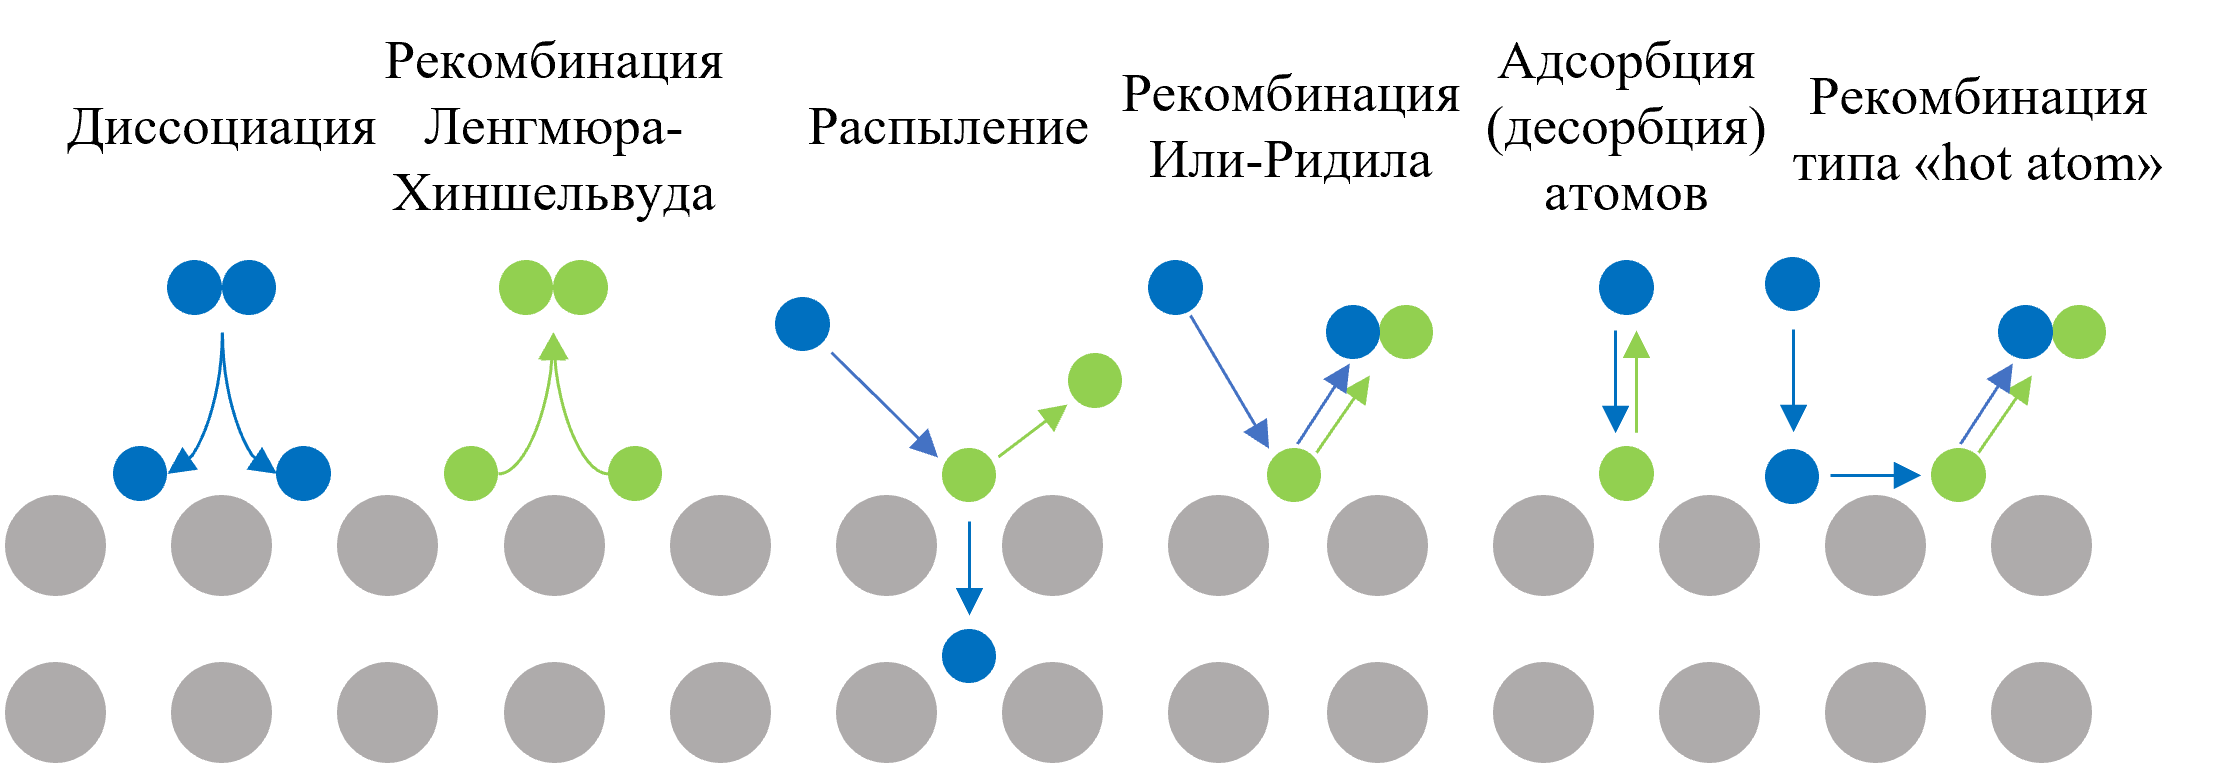
\includegraphics[scale=1]{surface_processes.png}
    }
    \caption{Схематическое представление некоторых процессы, происходящих на поверхности металла. Синие круги представляют падающие частицы (атомы или молекулы) из приповерхностной среды, зеленые круги соответствуют изначально адсорбированным атомам, серые "--- атомам материала поверхности}\label{fig:ch1/surface_processes}
\end{figure}

\begin{equation}
    K_\mathrm{S}=\cm \sqrt{P}
\end{equation}

\subsection{Закономерности накопления при стационарном плазменном облучении}

\subsubsection{Влияние потока}

\subsubsection{Влияние дозы}

\subsubsection{Влияние гелия}

\subsection{Влияние импульсных нагрузок на накопление}

\subsubsection{Импульсные тепловые нагрузки}

\subsubsection{Импульсные плазменные нагрузки}

\section{Методы дистанционного контроля содержания изотопов водорода в ОПЭ}\label{sec:ch1/sec5}

Стандартные методы контроля
Типы: ЛИД, ЛИДС, ЛИАС, ЛИИС
ЛИД
Апробация методик

\section{Выводы к Главе~\ref{ch:ch1}}\label{sec:ch1/sec6}

Для теста~\autocite{Kulagin2022a_rus}


\FloatBarrier
